\documentclass{article}
\usepackage{graphicx}
\usepackage{amsmath}
\graphicspath{ {Desktop/} }
\usepackage[utf8]{inputenc}
\title{\textbf{On the derivation of the contact width for two cylinders\thanks{With paralell axes}  in compression\thanks{Equal external compressive forces}}}
\author{\textit{R Surya Narayan}\\Department of Mechanical Engineering\\ Roll No. 111118091}
\date{27th March 2021}
\begin{document}
\maketitle
\section{Introduction}
This is a modest attempt in understanding the derivation behind the half width of two cylinders in compression with parallel axes. The derivation present in the book "Contact Mechanics" by K.Johnson (Cambridge University Press) has been reproduced with sufficient reasoning to bridge the heuristics of the problem and the complex mathematics that eventually manifests in the process of derivation. Though not original, an attempt is made to explain the reasoning behind each step. I hope this suffices the challenge thus put forth, considering a completely original derivation from scratch using the first principles of Engineering Mechanics would be rigorous and will require sufficient mathematical skill. The present reproduction from the said reference itself requires one to know a considerable number of topics in the theory on Contact Mechanics, namely, Hertzian stresses, point loading of elastic half-spaces and its associated integro-differential equations. In the said reference this has been presented over a series of chapters and comes together in \textit{Chapter 4-Normal Contact of elastic solids: Hertzian theory}. One would require to study \textit{Chapter-2:Line loading of elastic half-spaces} which expounds more on the general solutions to deformations for bodies in non-conformal contact. An attempt has been made to straighten this derivation out and filter the unnecessary parts for readers so that he/she is taken right from the first principles to the intended expression in the end. Before I proceed I would like to touch up what elastic half-spaces and non-conformal contacts mean as they might appear new to a reader first stumbling on this derivation.An \textit{elastic half-space} can simply be thought of as an infinite plane with elastic properties on which some deforming load acts. Half here refers to the lower half which on which the loads are supposed to act. \textit{Non-conformal} on the other hand simply refers to surfaces that don't perfectly mesh with each other on contact and hence some distance exists between the two surfaces over some small patch, if magnified over the contact point/line. On this note, I would like to proceed with the derivation from chapter 2 onwards from the book.  
\section{Line loading of a simple elastic half-space}
The following figure is a representation of a half-space, which is essentially infinite in the \textit{x} direction. One may wonder as to why the derivation is started from this point onwards. The answer to this question is quite simple. The following case, represents the simplest configuration one may encounter in the area of contact. Every other case maybe simplified without much loss of generality, to this simple case, and hence can be a good starting point to derive the final equation we are hunting for. This also forms the basis for vast part of Contact Mechanics.   
\begin{figure}[h]
 \centering
 \includegraphics{halfspace}
 \caption{An elastic half-space}
 \label{Figure 1:}
\end{figure} 
The symbols carry their usual meaning here. For this particular loading type, the governing differential equation is obtained in general form from the Theory of Elasticity. These are essentially equilibrium equations throughout the solid and can be obtained by equating the net moment and stress equal to zero for a small element as shown in the inset above. One can hence obtain:
\[
\frac{\partial \sigma_i}{\partial x_i} + \frac{\partial \tau_{x_i x_j}}{\partial x_j}=0 \tag{1} \label{eq:1}
\]
Where we have adopted: 
\[
x_1 = x, x_2 = z \tag{1.a} 
\]
Strains and displacements can be related using: 
\[
\epsilon_i = \frac{\partial u_i}{\partial x_i} \tag{2} \label{eq:2}
\]
\[
\gamma_{xz} = \frac{\partial u_x}{\partial x} + \frac{\partial u_z}{\partial z} \tag{3} \label{eq:3}
\]
Hooke's law can be used to relate the stresses to the strain  and one ends up with a bi-harmonic differential equation in \textit{x} and \textit{z} for a "stress potential function" $\phi(x,z)$ defined as: 
\[
\sigma_i = \frac{\partial^2 \phi}{\partial x_i^2}, \sigma_{xz} = -\frac{\partial^2 \phi}{\partial x \partial z} \tag{4} \label{eq:4}
\]
One can hence prove the subsequent bi-harmonic differential equation is:
\[
\nabla^2(\nabla^2 \phi) = 0 \tag{5} \label{eq:5}
\]
using the equilibrium equations \eqref{eq:1} and the strain relations \eqref{eq:2} and \eqref{eq:3}. One can now impose the boundary condition that the plane is loaded only in the region [\textit{-b,a}] and is identically zero everywhere else. These loads will correspond to the functions $p(x)$ and $q(x)$ respectively in the $z$ and the $x$ directions. A full derivation of the strains relating to the stresses and the subsequent equation is an exercise in the first principles of Engineering Mechanics and is currently  not included to preserve a certain degree of coherence and scope. Now once we have the governing differential equation ready, the next step is simply to explore the relevant loading cases and look at some general solutions to some common loads. This is carried out in the next section. Yet again, for the sake of simplicity, the solutions are just presented instead of a full solution owing to mathematical convolutions.
\subsection{A general solution to the bi-harmonic PDE}
In this section I just present a general solution to the PDE represented by \eqref{eq:5}.For a detailed derivation of the solutions the reader is referred to sections 2.2, 2.3 and 2.4 of the reference [1]. For the loading configuration shown below in \eqref{Figure 2:} the solutions to the stresses $\sigma_x$, $\sigma_z$ and $\tau_{xz}$ is obtained as integrals (6), (7), (8). To obtain the exact distributions of the stresses, one needs to know the distribution functions $p(x)$ and $q(x)$ respectively, the normal and the shear loading functions. However, even one without profound mathematical knowledge realizes that a complete closed form solution to such an integral is definitely not easy. Hence, one can switch to the usage of numerical integration to carry this out for more complicated loading cases. 
\begin{figure}[h]
 \centering
 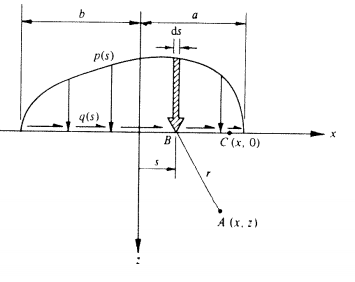
\includegraphics{distributed}
 \caption{Distributed loading}
 \label{Figure 2:}
\end{figure}  
To find out the strains as functions of $x$ one can differentiate under the integral sign of the displacements in (9) (10) to obtain the strain distributions (11) (12) (14)following equations \eqref{eq:2} and \eqref{eq:3}. 
\[
\sigma_x = -\frac{2z}{\pi}\int_{-b}^{a}\frac{p(s)(x-s)^2}{((x-s)^2+z^2)^2},ds - \frac{2}{\pi}\int_{-b}^{a}\frac{q(s)(x-s)^3}{((x-s)^2+z^2)^2}\,ds \tag{6} \label{eq:6}
\]
\[
\sigma_z = -\frac{2z^3}{\pi}\int_{-b}^{a}\frac{p(s)}{((x-s)^2+z^2)^2},ds - \frac{2z^2}{\pi}\int_{-b}^{a}\frac{q(s)(x-s)}{((x-s)^2+z^2)^2}\,ds \tag{7} \label{eq:7}
\]
\[
\tau_{xz} = -\frac{2z^2}{\pi}\int_{-b}^{a}\frac{p(s)(x-s)}{((x-s)^2+z^2)^2},ds - \frac{2z^2}{\pi}\int_{-b}^{a}\frac{q(s)(x-s)^2}{((x-s)^2+z^2)^2}\,ds \tag{8} \label{eq:8}
\]
\[
\frac{\partial u_x}{\partial x} = -p(x)\frac{(1-2\nu)(1+\nu)}{E}-\frac{2(1-\nu^2)}{\pi E} \int_{-b}^{a}\frac{q(s)}{(x-s} \tag{9} \label{eq:9}
\]
\[
\frac{\partial u_z}{\partial z} = -\frac{2(1-\nu^2)}{\pi E}{\int_{-b}^{a}\frac{p(s)}{x-s}ds}-\frac{(1-2\nu)(1+\nu)}{E}q(x) \tag{10} \label{eq:10}
\]
\subsection{The Hertzian theory}
We now move closer to the problem we intend to solve. Consider two non-conformal bodies in contact. Initially they are in contact with each other at exactly one point or along a single line. There is some separation between the two surfaces $h$ which varies along with the $x$ axis in the non-deformed state. This can be trivially derived using principles of coordinate geometry to be a parabolic function as follows: 
\[
h = \frac{1}{2}(\frac{1}{\rho_1} + \frac{1}{\rho_2})x^2 = \frac{x^2}{2\rho_eq} \tag{12}
\]
Now consider a force $P$ applied on either of the cylinders due to which they deflect $\delta_1$ and $\delta_2$ into each other. To keep track of things, consider two surface points $S_1(x,y,z_1)$ and $S_2(x,y,z_2)$ which were separated by $h$ given by (12). The surfaces are each displaced by an amount $u_z1$ and $u_z2$. 
Hence based on the Figure 3 one may write:
\[
u_z1 + u_z2 + h = \delta_1 + \delta_2 \tag{13} \label{eq:13}
\]
For convenience, set $\delta = \delta_1 + \delta_2$. Hence we get: 
\[
u_z1 + u_z2 = \delta - h = \delta - \frac{x^2}{2\rho_e q} \tag{14} \label{eq:14}  
\]
\begin{figure}[h]
 \centering
 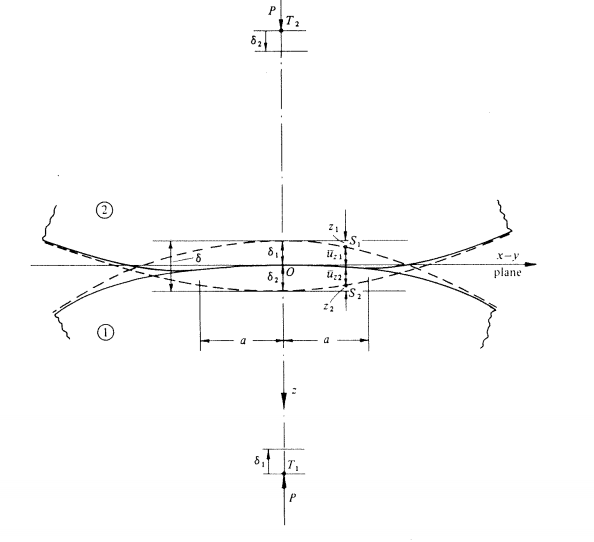
\includegraphics{contact_zone}
 \caption{Contact Zone: magnified view}
 \label{Figure 3:}
\end{figure}
As abundantly clear from the figure, we define $2a$ to be the contact patch/width overwhich the above relations hold. We now introduce the Hertzian theory of contact stresses to formulate the elasticity problem under the following assumptions: 
\begin{enumerate}
\item The surfaces are non-conforming and continuous, $a<<R_i$
\item Each solid is considered a half-space
\item The surfaces are frictionless
\end{enumerate}
We hence have to find out the distribution of the pressure $p(x,y)$ over the contact area $S$ in the two half-spaces such that the displacements that follow from the solution abide by equation \eqref{eq:14}. This is termed the Hertzian stress formulation, which Hertz developed when pondering over interference fringes over surfaces in contact, one fine Christmas evening! So now that we have all our elements lined up we are ready for the actual derivation. 
\subsection{The expression for the contact width}
We now use equation \eqref{eq:10} for bodies 1 and 2 neglecting the tangential stress $q(x)$ to get: 
\[
\frac{\partial u_{z1}}{\partial x} + \frac{\partial u_{z2}}{\partial x} = -\frac{2(1-\nu_1^2)}{\pi E_1}{\int_{-a}^{a}\frac{p(s)}{x-s}ds} -\frac{2(1-\nu_2^2)}{\pi E_2}{\int_{-a}^{a}\frac{p(s)}{x-s}ds} \tag{15} \label{eq:15} 
\]
\eqref{eq:15} can be re-written as: 
\[
\frac{\partial u_{z1}}{\partial x} + \frac{\partial u_{z2}}{\partial x} = -(\frac{2(1-\nu_1^2)}{\pi E_1}+\frac{2(1-\nu_2^2)}{\pi E_2}){\int_{-a}^{a}\frac{p(s)}{x-s}ds} \tag{16} \label{eq:16}
\]
This is often simplified by introducing $E^*$ as follows: 
\[
\frac{\partial u_{z1}}{\partial x} + \frac{\partial u_{z2}}{\partial x} = -(\frac{2}{\pi E^*}){\int_{-a}^{a}\frac{p(s)}{x-s}ds} \tag{17} \label{eq:17}
\] 
Now differential \eqref{eq:14} to get: 
\[
\frac{\partial u_{z1}}{\partial x} + \frac{\partial u_{z2}}{\partial x} = -\frac{x}{\rho_{eq}} \tag{18} \label{eq:18}
\] 
Equating \eqref{eq:18} and \eqref{eq:17} we may write: 
\[
{\int_{-a}^{a}\frac{p(s)}{x-s}ds} = \frac{\pi E^*x}{2 \rho_{eq}} \tag{19} \label{eq:19}
\]
This is an integral equation, the solutions to which are discussed in the section 2.7 of the reference. The solution is just stated here for simplicity sake: 
\[
p(x) = -\frac{\pi E^*}{2\rho_{eq}}\frac{x^2-0.5a^2}{\pi \sqrt{(a^2-x^2})} + \frac{P}{\pi (\sqrt{a^2-x^2})} \tag{20} \label{eq:20}
\]
Imposing the condition that the pressure must be positive everywhere, we obtain that:
\[
P\geq\frac{\pi a^2 E*}{4\rho_{eq}} \tag{21} \label{21}
\]
However, if the pressure shoots beyond the computed value above, we observe that expression for $p(x)$ possesses a singularity (i.e. rises to infinite) at $x=a$. Hence the equality holds in \eqref{21} giving us the desired result: 
\[
2a = \sqrt{\frac{16P\rho_{eq}}{\pi E^*}} \tag{22} 
\]
\end{document}